\documentclass[12pt]{article}
\usepackage{natbib}
\usepackage{eso-pic}
\usepackage{amsmath} % flere matematikkommandoer
\usepackage{amssymb}
\usepackage[utf8]{inputenc} % æøå
\usepackage[T1]{fontenc} % mere æøå
\usepackage[danish]{babel} % orddeling
\usepackage{verbatim} % så man kan skrive ren tekst
\usepackage[a4paper, margin = 1in]{geometry}
\usepackage{graphicx}
\usepackage{booktabs}
\usepackage{enumitem}
\usepackage{placeins}
\author{
  Christian Kjær Larsen\\
  \texttt{011292} \\[.4cm]
  Lukas Svarre Engedal\\
  \texttt{210790} \\[.4cm]
  Tobias Sønderskov Hansen\\
  \texttt{243095} \\[.4cm]
  Instruktor: Aske Mottelson\\[.4cm]
  \vspace{10cm}
}

\title{
  \vspace{3cm}
  \Huge{ProjDat 2015} \\[.25cm]
  \large{Delrapport 2}
}

\begin{document}

\AddToShipoutPicture*{\put(0,0){\includegraphics*[viewport=0 0 700 600]{includes/nat-farve}}}
\AddToShipoutPicture*{\put(0,602){\includegraphics*[viewport=0 600 700 1600]{includes/nat-farve}}}

%% Change `ku-en` to `nat-en` to use the `Faculty of Science` header
\AddToShipoutPicture*{\put(0,0){\includegraphics*{includes/nat-en}}}

\clearpage\maketitle
\thispagestyle{empty}

\newpage

\tableofcontents %generate table of content

\thispagestyle{empty}

\newpage
\pagestyle{plain}
\setcounter{page}{1}
\pagenumbering{arabic}

\section{Abstract}
\label{sec:abstract}

\section{Formål og rammer}
\label{sec:formal_og_rammer}
I dette afsnit beskrives systemets formål og rammer ved \textit{FACTOR}-kriteriet.
\begin{description}
    \item[Funktionalitet]
        Besvare og oprette programmeringsspørgsmål, Analysere de studerendes fremskridt.
    \item[Anvendelsesområde]
        Loginsystem, Spørgsmålshåndtering, Spørgsmålsbesvarelse, Analyse.
    \item[Betingelser]
        Undervisere har begrænsede resurser. Studerende har svært ved programmering.
    \item[Teknologi]
        Webapplikation med teknologi der er nemt at sætte sig ind i.
    \item[Objekter]
        Studerende, Spørgsmål, Hints, Undervisere.
    \item[Ansvar]
        E-læringssystem til hjælp af studerende med programmering.
\end{description}
\section{Kravspecifikation}
\label{sec:kravspecifikation}

\subsection{Krav}
\label{sub:krav}
\paragraph{Funktionelle krav}
De funktionelle krav for systemet er i tråd med afsnit 4.3.1 i \cite{OOSE}, nemlig at de omhandler den specifikke brug af systemet.
\begin{itemize}
    \item Systemet skal være en hjemmeside med opgaver, som kan løses individuelt af studerende.
    \item Der kræves login, så man kan følge med i den studerendes udvikling.
    \item Spørgsmålene skal være grupperede efter hvilke læringsmål de tester.
    \item Læringsmålene skal igen grupperes efter et \emph{threshold}, som er et øvre læringsmål hvorefter der kommer sværere stof.
    \item Der skal være hints til opgaverne, og der skal kunne gives feedback til hints.
    \item Alle forsøg på opgavebesvarelser skal gemmes i en log.
\end{itemize}
Hvis der er tid i en af de senere iterationer, så er der en række ekstra krav som kan implementeres.
\begin{itemize}
    \item Loggen skal bruges til at give underviseren information om hvilke spørgsmål der er svære.
    \item Der skal tilføjes en grad af \emph{gamification}, så der gives badges og point for fremskridt, og det bliver muligt at følge med i andres fremskridt.
    \item Hvis man ikke har øvet sig i et emne i et stykke tid, så falder ens erfaring i området.
\end{itemize}

\paragraph{Ikke-funktionelle krav}
\label{par:ikke_funktionelle_krav}
I afsnit 4.3.2 i \cite{OOSE} beskrives ikke-funktionelle krav som krav, der ikke direkte beskriver funktionaliteten, men mere generelle krav omkring ting som brugervenlighed, ydeevne, pålidelighed og hvor vedligeholdesesvenligt systemet er. De ikke-funktionelle krav til dette projekt er forholdsvis begrænsede, idet vi har fået ret stor frihed i forhold til hvordan vi løser opgaven af vores kunde.

Det vigtigste krav er at det skal være nemt at tilføje nye opgaver til systemet, sådan at kursuslederne efterfølgende kan opbygge en tilstrækkelig samling af opgaver til de studerende. Derudover er det også et mere overordnet krav at det endelige produkt gerne skal være så simpelt og modulært som muligt, sådan at det er nemt at overtage, udvide og bygge videre på efter at vi overgiver projektet til kunden. Ingen af kunderne er web-udviklere, så det er også vigtigt at det valgte framework er veldokumenteret og rimeligt simpelt at bruge.

\subsection{Use case model}
\label{sub:use_case_model}
\begin{figure}[htpb]
  \centering
  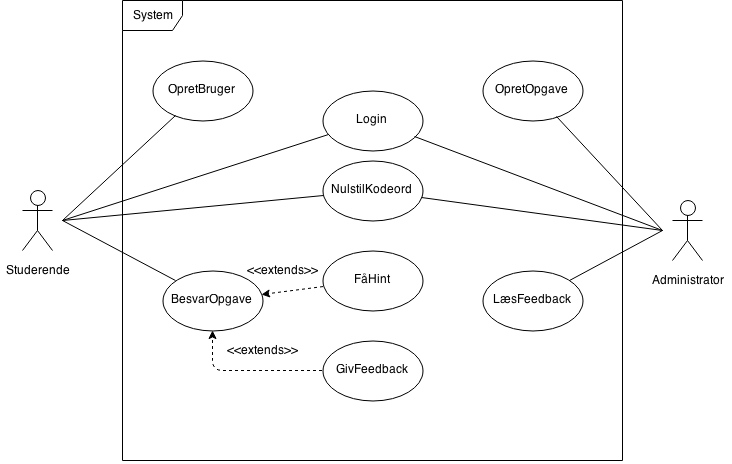
\includegraphics[width=0.8\linewidth]{figures/UseCaseModel.png}
  \caption{Use case model for vores system.}
  \label{fig:use_case_model}
\end{figure}
På Figur \ref{fig:use_case_model} kan man se vores use case model diagram. Vi har at gøre med to aktører, nemlig studerende og administratorer. Det vigtige for studerende er at de kan oprette sig på siden, og at de har adgang til opgaver de kan besvare. Det vigtige for administratorer er at de kan administrere opgaverne, og at de kan få feedback og statistik på hvordan de studerende klarer opgaverne. Begge aktører skal desuden kunne benytte simpel funktionalitet i forbindelse med deres login.

\subsection{Use cases}
\label{sub:use_cases}

\begin{figure}[htpb]
    \centering
    \begin{tabular}{r p{10cm}}
        \toprule
        \textit{Navn på use-case:} & \verb!OpretBruger! \\
        \hline
        \textit{Deltagende aktører:} & Påbegyndt af en studerende \\
        \hline
        \textit{Hændelser:} & \begin{enumerate}[nolistsep]
            \item En studerende åbner hjemmesiden og klikker på \verb!register!
            \item Den studerende indtaster sine brugeroplysninger, dvs. ku-id og løsen.
            \item Systemet opretter brugeren, og sender en e-mail med et aktiveringslink.
            \item Den studerende klikker på linket, og kontoen aktiveres.
            \item Den studerende bringes til login-siden.
            \item Den studerende indtaster ku-id og løsen og klikker \verb!Login!
            \item Der informeres om succesfuldt login, og brugeren bringes til applikationen.
        \end{enumerate}  \\
        \hline
        \textit{Startbetingelse:} & En studerende har ingen konto, og er ikke logget ind. \\
        \hline
        \textit{Slutbetingelse:} & En studerende har en aktiveret konto og er logget ind. \\
        \bottomrule
    \end{tabular}
    \caption{Use case omkring opretning af brugere.}
    \label{fig:use_case1}
\end{figure}

\begin{figure}[htpb]
    \centering
    \begin{tabular}{r p{10cm}}
        \toprule
        \textit{Navn på use-case:} & \verb!BesvarOpgave! \\
        \hline
        \textit{Deltagende aktører:} & Påbegyndt af en studerende \\
        \hline
        \textit{Hændelser:} & \begin{enumerate}[nolistsep]
            \item En studerende åbner hjemmesiden.
        \end{enumerate}  \\
        \hline
        \textit{Startbetingelse:} & En studerende der er logget ind. \\
        \hline
        \textit{Slutbetingelse:} & En studerende der er logget ind og har besvaret en opgave. \\
        \bottomrule
    \end{tabular}
    \caption{Use case omkring besvarelse af opgaver.}
    \label{fig:use_case1}
\end{figure}

\begin{figure}[htpb]
    \centering
    \begin{tabular}{r p{10cm}}
        \toprule
        \textit{Navn på use-case:} & \verb!OpretOpgave! \\
        \hline
        \textit{Deltagende aktører:} & Påbegyndt af en administrator \\
        \hline
        \textit{Hændelser:} & \begin{enumerate}[nolistsep]
            \item En studerende åbner hjemmesiden.
        \end{enumerate}  \\
        \hline
        \textit{Startbetingelse:} & En administrator der er logget ind. \\
        \hline
        \textit{Slutbetingelse:} & En administrator der er logget ind og har oprettet en opgave. \\
        \bottomrule
    \end{tabular}
    \caption{Use case omkring besvarelse af opgaver.}
    \label{fig:use_case1}
\end{figure}

\subsection{Klassediagram}
Ikke implementeret

\subsection{BCE-model}
\begin{figure}[htpb]
  \centering
  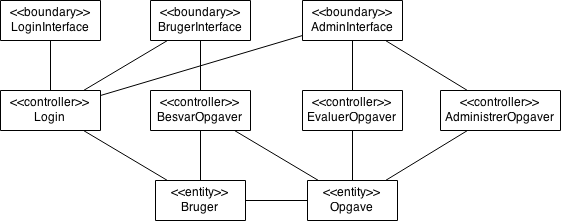
\includegraphics[width=0.8\linewidth]{figures/BCE-Model.png}
  \caption{BCE model for vores system.}
  \label{fig:bce_model}
\end{figure}
På Figur \ref{fig:bce_model} kan man se vores BCE model. Modellen har to entity-objekter, fire controller-objekter samt tre boundary-objekter. \\
De to entity-objekter er \verb!Bruger! og \verb!Opgave!. \verb!Bruger! indeholder informationer om hver enkelt bruger som login-oplysninger, hvor vidt brugeren er en studerende eller en admin samt hvilke opgaver brugeren allerede har løst. \verb!Opgave! indeholder alle informationerne om de enkelte opgaver, det er både selve opgaven der skal løses samt statistik omkring hvordan det er gået når studerende har løst opgaven. \\
Modellen har tre boundary-objekter, hvor det første man vil støde på er \verb!login!-brugergrænsefladen, der sammen med \verb!login!-controlleren sørger for at logge brugerne ind i systemet. Derefter vil man så enten have adgang til \verb!Bruger!-grænsefladen eller \verb!Admin!-grænsefladen afhængig af hvad ens status er, og derfra har man adgang til en række controllers. \\
Modellen har fire controller-objekter, hvor den første er \verb!login!-controlleren der som tidligere nævnt står for at logge brugere ind i systemet. Som studerende vil man have adgang til \verb!BesvarOpgave!-controlleren, der snakker sammen med \verb!Bruger! og \verb!Opgave! og sørger for at stille brugeren de rigtige opgaver. Som admin vil man have adgang til to controllers, nemlig \verb!EvaluerOpgave!-controlleren og \verb!AdministrerOpgave!-controlleren. \verb!EvaluerOpgave!-controlleren snakker sammen med \verb!Opgave! og giver en adgang til de forskellige slags statistik der bliver samlet om opgaverne, og \verb!AdministrerOpgave!-controlleren snakker ligeledes sammen med \verb!Opgave! og giver en adgang til at slette eller ændre i eksisterende opgaver samt tilføje nye.

\subsection{Sekvens-diagrammer}
Ikke implementeret

\section{Systemdesign}
\label{sec:systemdesign}
Ikke implementeret

\section{Program- og systemtest}
\label{sec:program_og_systemtest}
Ikke implementeret

\section{Brugergrænseflade og interaktionsdesign}
\label{sec:brugergraenseflade}
Ikke implementeret

\section{Projektsamarbejdet}
\label{sec:projektsamarbejdet}
Ikke implementeret

\appendix
\section{Versionsstyring}

\section{Changelog}
\begin{tabular}{l l l}
08-04-2015 & CKL & Dokument oprettet \\
14-04-2015 & CKL & Tilføjet use cases og krav \\
16-04-2015 & LSE & Tilføjet UseCaseModel og BCE model \\
\end{tabular}

\section{Timeline}
\begin{tabular}{l l p{8cm}}
11-03-2015 & Første møde med kunde: & Vi har første møde med kunden hvor vi snakker om hvad projektet går ud på og diskuterer krav og løsningsforslag.
\end{tabular}

\bibliographystyle{alpha}
\bibliography{refs}{}

\end{document}
